\documentclass[]{spie}  %>>> use for US letter paper
%\documentclass[a4paper]{spie}  %>>> use this instead for A4 paper
%\documentclass[nocompress]{spie}  %>>> to avoid compression of citations

\renewcommand{\baselinestretch}{1.0} % Change to 1.65 for double spacing
 
\usepackage{amsmath,amsfonts,amssymb}
\usepackage{graphicx}
\usepackage[colorlinks=true, allcolors=blue]{hyperref}
\usepackage{glossaries}
\title{Simulating the Effects of Exozodiacal Dust in WFIRST CGI observations}

\author[a]{Ewan S. Douglas}
\author[b]{John Debes}
\author[a]{Kian Miliani}
\affil[a]{University of Arizona, Tucson, AZ, USA}
\affil[b]{STScI, Baltimore, MD, USA}

\authorinfo{Further author information: (Send correspondence to A.A.A.)\\A.A.A.: E-mail: aaa@tbk2.edu, Telephone: 1 505 123 1234\\  B.B.A.: E-mail: bba@cmp.com, Telephone: +33 (0)1 98 76 54 32}

% Option to view page numbers
\pagestyle{empty} % change to \pagestyle{plain} for page numbers   
\setcounter{page}{301} % Set start page numbering at e.g. 301
 
\begin{document} 
\maketitle

\begin{abstract}

\end{abstract}

% Include a list of keywords after the abstract 
\keywords{Manuscript format, template, SPIE Proceedings, LaTeX}

\section{INTRODUCTION}
\label{sec:intro}  % \label{} allows reference to this section
Exozodiacal dust presents 
\begin{figure}
    \centering
    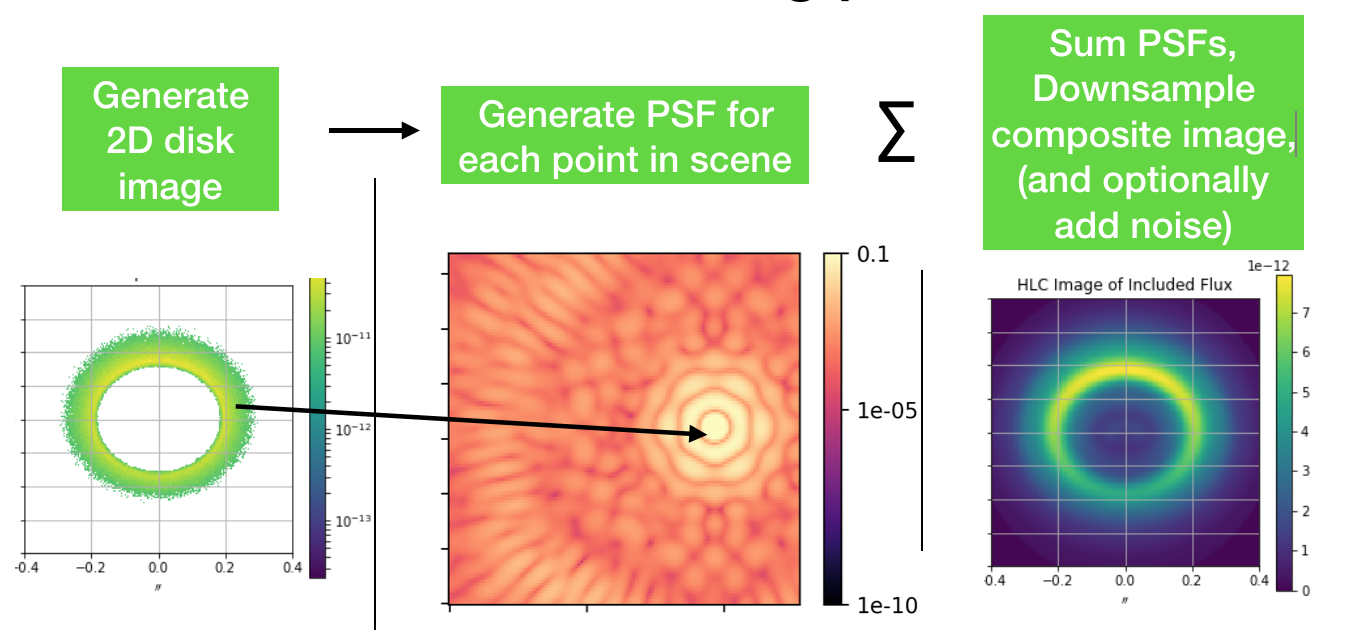
\includegraphics[width=0.95\textwidth]{flow.png}
    \caption{Simulation flow for field dependant PSF simulations of debris disks.}
    \label{fig:my_label}
\end{figure}
\section{Methods}



\section{Preliminary Results}

    
\acknowledgments % equivalent to \section*{ACKNOWLEDGMENTS}   
The authors acknowledge valuable inputs from  Vanessa Bailey,  Brian Kern, John Krist, Hanying Zhou,   and the rest of the JPL CGI team.
 Support for this work was provided by the WFIRST Science Investigation team prime award \#NNG16PJ24C.
This work was also supported by the Arizona Board of Regents Technology Research
Initiative Fund (TRIF).
This research made use of the \gls{MGHPCC} via MIT Research Computing and High Performance Computing (HPC) resources supported by the University of Arizona (UA) TRIF, UITS, and RDI and maintained by the UA Research Technologies department.

% References
%\bibliography{report} % bibliography data in report.bib
\bibliographystyle{spiebib} % makes bibtex use spiebib.bst

\end{document} 
